%%%%%%%%%%%%%%%%%%%%%%%%%%%%%%%%%%%%%%%%%
% Thin Sectioned Essay
% LaTeX Template
% Version 1.0 (3/8/13)
%
% This template has been downloaded from:
% http://www.LaTeXTemplates.com
%
% Original Author:
% Nicolas Diaz (nsdiaz@uc.cl) with extensive modifications by:
% Vel (vel@latextemplates.com)
%
% License:
% CC BY-NC-SA 3.0 (http://creativecommons.org/licenses/by-nc-sa/3.0/)
%
%%%%%%%%%%%%%%%%%%%%%%%%%%%%%%%%%%%%%%%%%

%----------------------------------------------------------------------------------------
%	PACKAGES AND OTHER DOCUMENT CONFIGURATIONS
%----------------------------------------------------------------------------------------

\documentclass[a4paper, 11pt]{article} % Font size (can be 10pt, 11pt or 12pt) and paper size (remove a4paper for US letter paper)
\usepackage[inner=2cm,outer=2cm]{geometry} %left=4cm,right=2cm would be equivalent

\usepackage[protrusion=true,expansion=true]{microtype} % Better typography
\usepackage{graphicx} % Required for including pictures
\usepackage{wrapfig} % Allows in-line images
\usepackage{subfigure}
\usepackage{amsmath}
\usepackage{mathpazo} % Use the Palatino font
\usepackage[T1]{fontenc} % Required for accented characters
\usepackage[toc,page]{appendix}
\newcommand{\sqlen}[1]{\ensuremath{(x - x_{#1})^2 + (y-y_{#1})^2}}
\newcommand{\rili}[1]{\ensuremath{\frac{r_{#1}^2}{l_{#1}}}}
\linespread{1.05} % Change line spacing here, Palatino benefits from a slight increase by default

\makeatletter
\renewcommand\@biblabel[1]{\textbf{#1.}} % Change the square brackets for each bibliography item from '[1]' to '1.'
\renewcommand{\@listI}{\itemsep=0pt} % Reduce the space between items in the itemize and enumerate environments and the bibliography

\renewcommand{\maketitle}{ % Customize the title - do not edit title and author name here, see the TITLE block below
\begin{flushright} % Right align
{\LARGE\@title} % Increase the font size of the title

\vspace{50pt} % Some vertical space between the title and author name

{\large\@author} % Author name
\\\@date % Date

\vspace{40pt} % Some vertical space between the author block and abstract
\end{flushright}
}

%----------------------------------------------------------------------------------------
%	TITLE
%----------------------------------------------------------------------------------------

\title{\textbf{Constrained Constructive Optimization implementation}\\ % Title
Reproducing Rudolph Karch paper} % Subtitle

\author{\textsc{Clara Jaquet} % Author
\\{\textit{Paris-Est University}}} % Institution

\date{\today} % Date

%----------------------------------------------------------------------------------------

\begin{document}

\maketitle % Print the title section

%----------------------------------------------------------------------------------------
%	ABSTRACT AND KEYWORDS
%----------------------------------------------------------------------------------------

%\renewcommand{\abstractname}{Summary} % Uncomment to change the name of the abstract to something else

\begin{abstract}
Implement CCO in 2D, then 3D based on Karch's work \cite{karch1999three}. In another step consider implementation for convex volume. 
Combination of CFD laws, geometry, and optimization. Encapsulated articles : requires summary in one paper.
\end{abstract}

\hspace*{3,6mm}\textit{Keywords:} constrained constructive optimization, implementation % Keywords

\vspace{30pt} % Some vertical space between the abstract and first section

\tableofcontents
%----------------------------------------------------------------------------------------
%	ESSAY BODY
%----------------------------------------------------------------------------------------

\section*{Introduction}

Constrained constructive optimization consists of growing a tree governed by minimizing a target function. 

In Karch's method the tree is constrained into a given convex perfusion volume, and the target function minimizes the total tree volume during growth. Segment are added one by one and fulfill both local optimization (single bifurcation scale) and global optimization (tree scale). The local optimization is based on Kamiya's work \cite{kamiya1972optimal}, whereas the global optimization has been implemented first by Schreiner in 2D \cite{schreiner1993computer}. 

\section{Global optimization}

Initialization of the method requires physiological parameters inputs, and a randomized starting point.

Then Karch's protocol consists of a complete loop for each added segment. A  random location is picked under some constraints (geometry and physiology), to use it as a segment end candidate. Its connection is tested with neighbor segments, producing a bifurcation under topological, structural and functional constraints. In view of this new branch impact on the whole tree (induced by fluid mechanics laws), the optimal connection is selected according to a target function (minimal volume of the total tree). 


\subsection{Assumptions and boundary conditions}
The vascular tree is grown under specific assumptions and boundary conditions.

The perfused volume is convexe and supposed homogeneously filled. The terminal segments correspond to pre-arteriole level, that feed a non modeled micro-vasculature.
The blood is an incompressible, homgeneous Newtonian fluid, studied at steady state and in laminar flow conditions. 

The resistance and the pressure drop of a segment $j$ are defined by:
\begin{equation}\label{resistance}
R_j = \frac{8\mu}{\pi}\frac{l_j}{r_j^4} \text{ with } \mu \text{ the viscosity }
\end{equation}
\begin{equation}\label{Pdrop}
\Delta P_j = R_j Q_j
\end{equation}
The total resistance of the tree is calculated recursively by tree decomposition, considering parallel and serial arrangements.

The physiological parameters are defined such as in the following table:\\

The pressure at distal end of terminal segment,$P_{term}$, are equal and inflow pressure to the micro-circulation.
The terminal flows $Q_{term,j}$ are equals, and delivered into the micro-circulation agains $P_{term}$. Because of flow conservation their sum correspond to the perfusion flow at the root $Q_{perf}$. 
The laminar flow resistance of the whole tree induces a given total $Q_{perf}$ accross $\Delta P$.$Q_{perf}$ is the same for each step of the tree generation.

The tree grown is dichotomic, so that the total number of segments is calculated from:
\begin{equation}
N_{tot} = 2 N_{term} -1
\end{equation}

This tree follows Murray's law, with a coefficient equal to 3.

\subsection{Initialization step}  
Inputs:
\begin{itemize}
\item convexe perfusion surface or volume definition: position and shape
\item number of terminal segments, $N_{term}$
\item location of the root (in our case at the border of the perfusion territory)
\item a random location inside the perfusion territory for the first segment end 
\end{itemize}

\subsection{Loop to add new segment}
We are provided a new location, $n_loc$, and want to find its optimal connection to the existing tree. For this purpose we select the $N_con$ closest existing segments to this location, compute a local optimization for each of them, then evaluate the connection impact on the whole tree, and as a global optimization process, we determine the one minimizing best the total tree volume.

\subsubsection{Constrained new location $n_loc$}
A random position is picked, that has to fulfill two constraints: belong to the perfusion territory and respect a distance criterion. 
This criterion is defined based on the final and current size of the tree:
\begin{equation}
d_{thresh} = (\pi r_{supp}^2 / k_{term})^\frac{1}{2}
\end{equation}
with $k_{term}$ the number of terminal segment at the current step, and $r_{supp}$ defined from  the estimated size of a micro-circulatory black-box area, knowing the total perfused area $A_{perf}$:
\begin{equation}
\pi r_{supp}^2 = A_{perf} / N_{term}
\end{equation}
In 3D this criteria is defined as:
\begin{equation}
d_{thresh} = (\frac{4}{3} \pi r_{supp}^3 / k_{term})^\frac{1}{3}
\end{equation}
with
\begin{equation}
\frac{4}{3}\pi r_{supp}^3 = V_{perf} / N_{term}
\end{equation}
This distance criteron is updated after each new segment is added, so that it decreases during tree growth. If no location is found that respect this distance to existing segments within the perfusion territory, then the distance criteria is multiplied by 0.9 and the process repeated until a new position is found that fulfills both constraints. 
In the following steps, we will call... the parent and children segments.

\subsubsection{Test local connection}

For each neighbor segment of $n_loc$ we calculate what would be the optimal connection to $n_loc$ based on single bifurcation optimization established by Kamyia \cite{kamiya1972optimal}, and is fully detailed in \ref{Kamiya}. If this local optimization process is successful, we apply two additional checks:
\begin{itemize}
\item We control that the resulting segments are not degenerated ones, which means all three segments of the new bifurcations respect relationship between length and radius: $2r_i \leq l_i$

\item We control that none of the three resulting segments overlap any existing segment of the tree.
\end{itemize}

With this step we ensure the connection to be locally optimal and plausible for the tree.

\subsubsection{Propagate impact on whole tree}
By adding a new terminal segments, inducing a new generated bifurcation, we disturb the distribution of segmental flows. In order to reestablish the correct terminal flows, the hydrodynamic resistance of the tree must be adjusted. As the lengths of the segments as well as the terminal and perfusion pressures are fixed, this can only be accomplished by proper rescaling of the segment's radii.\\

If we define the reduced hydrodynamic resistance $R^*$ as $R^*_i = R_i r_i^4$ we can calculate the reduced hydrodynamic resistance of a segment including its left and right subtrees by recursively traversing the subtrees:
\begin{equation} \label{red resistance}
R^*_{sub,i} = \frac{8\mu}{\pi}l_j + \left( \frac{(r_{left,j}/r_j)^4}{R_{left,j}^*} + \frac{(r_{right,j}/r_j)^4}{R_{right,j}^*}\right)^{-1}
\end{equation}
Considering the assumptions \ref{Pdrop} and \ref{resistance}, we can then calculate the radius ratio of two children segments from resistance and flow:
\begin{equation} \label{children ratio}
\frac{r_i}{r_j} = \left(\frac{Q_iR_{sub,i}^*}{Q_jR_{sub,j}^*}\right)^\frac{1}{4}
\end{equation}
with $R_j$ and $Q_j$ the segment resistance.

Instead of storing the absolute radius for each segment, we consider the ratio between parent and its children: $\beta^i_k = r_i / r_k$ and $\beta^j_k = r_j / r_k$ with i and j the children, k the parent segment. Because of the tree respecting Murray's law, these ratios can actually be calculated directly from the ratio between children segments (see annexe for details):
\begin{equation}
\beta^i_k = \left( 1 + (\frac{r_i}{r_j})^{-\gamma}\right)^\frac{-1}{\gamma} \text{ and }
\beta^j_k = \left( 1 + (\frac{r_i}{r_j})^{\gamma}\right)^\frac{-1}{\gamma}
\end{equation}


Calculating the reduced resistance for each children with \ref{red resistance}, and knowing the flow, we obtain the children radius ratio from \ref{children ratio}, which is used to calculate $\beta$ values, stored with the parent segment properties. 
The subtrees distal to the new bifurcation remain constant and unaffected by the addition of the new branch, whereas upstream bifurcations are updated following this exact same process. By this methode, called "balancing of bifurcation ratios", the radius rescaling is propagated up the tree.
 


\subsubsection{Measure target function}
Calculate root radius from
\begin{equation}
r_{root} = \left( R_{sub, root}^* \frac{Q_{perf}}{P_{perf}-Q_{term}}\right)^\frac{1}{4}
\end{equation}
Measure total tree volume

\subsubsection{Select best connection between neighbors}
store result in cet: volume, betas, position

compare 

add the best one,then update flow, resistance, distance criteria and start again




\subsection{Example of results}
\subsubsection{2D}
\subsubsection{3D}
Output: images
decrease of radius, to maintain constant resistance


%------------------------------------------------

\section{Local optimization: single bifurcation scale}\label{Kamiya}
Kamiya proposes a numerical solution to determine minimum volume bifurcation under restriction of physiological parameters, determinant pressure and flow, and locations at origin and terminals.

This method built in 2D assumes the flow to be laminar and vessels are composed of straight ducts lying on a plane. 

Note: Karch found that the optimum positions of the bifurcations in their 3D model trees were always found to lie in the plane defined by the endpoints of the respective three neighboring segments, which is consistent with the literature \cite{zamir1986branching}. 


\subsection*{Process: iterative nested loops}

Defining a starting position as the convex average of origin and terminal locations, weighted by respective flows.
\begin{equation}
(x,y) = (\frac{f_0x_0 + f_1x_1 + f_2x_2}{2f_0},\frac{f_0y_0 + f_1y_1 + f_2y_2 )}{2f_0})
\end{equation}
Calculate each segment length.
\begin{equation}
l_i^2 = (x - x_i)^2 + (y - y_i)^2
\label{length}
\end{equation}
Numerically calculate the new radii $r_0$, $r_1$,$r_2$. These ones are expected to satisfy both Hagen-Poiseuille's law and volume minimization.

When location of origin and two terminals segments, their pressure, and their flows are given, according to Hagen - Poiseuille's law:
\begin{align}
&\Delta P_1 = P_1 - P_0 = \kappa(\frac{f_0l_0}{r_0^4} + \frac{f_1l_1}{r_1^4}), \\
&\Delta P_2 = P_2 - P_0 = \kappa(\frac{f_0l_0}{r_0^4} + \frac{f_2l_2}{r_2^4})
\label{poiseuille}
\end{align}
  
According to  Kamiya, differentiating the tree volume with $x$, $y$ and $r_0$ and equating them to zero, one obtains:
\begin{equation}
\frac{r_0^6}{f_0} = \frac{r_1^6}{f_1} + \frac{r_2^6}{f_2}
\label{min volume}
\end{equation}
and 
\begin{equation}
x = \frac{x_0 r_0^2/l_0 + x_1 r_1^2/l_1 + x_2 r_2^2/l_2}{r_0^2/l_0 + r_1^2/l_1 + r_2^2 / l_2},
y = \frac{y_0 r_0^2/l_0 + y_1 r_1^2/l_1 + y_2 r_2^2/l_2}{r_0^2/l_0 + r_1^2/l_1 + r_2^2 / l_2}
\label{position}
\end{equation}
The details of the path to these equations is provided in appendix.

Using $R = r^2$ in \eqref{min volume}, we can express $R_0$ as:
\begin{equation}
R_0^3 = f_0(\frac{R_1^3}{f_1} + \frac{R_2^3}{f_2})
\end{equation} 
Substituting this inside \eqref{poiseuille}, one obtains the non linear system:
\begin{align}
\begin{cases}
&\frac{\Delta P_1}{\kappa}R_1^2 \left(f_0(\frac{R_1^3}{f_1} + \frac{R_2^3}{f_2}) \right)^\frac{2}{3} -f_0l_0R_1^2 - f_1l_1\left(f_0(\frac{R_1^3}{f_1} + \frac{R_2^3}{f_2}) \right)^\frac{2}{3} = 0 \\
&\frac{\Delta P_2}{\kappa}R_2^2 \left(f_0(\frac{R_1^3}{f_1} + \frac{R_2^3}{f_2}) \right)^\frac{2}{3} -f_0l_0R_2^2 - f_2l_2\left(f_0(\frac{R_1^3}{f_1} + \frac{R_2^3}{f_2}) \right)^\frac{2}{3} = 0
\end{cases}
\label{non linear system}
\end{align}

We are looking for the root satisfying these equations using a non linear solver. If the solution converges, we get the new radii, that are needed to calculate the new position of the branching point in \eqref{position}. This locations is a new input for the loop to iterate again (calculating length \eqref{length}, then new radii \eqref{non linear system}, new location \eqref{position} and so on). 
If this iterative loop converges and the bifurcation total volume decreases, the bifurcation is solved and provided with optimal radii and position.

Note: in CCO the pressure is not determined all along vessels (only at the root and terminal segments). In order to adapt to our situation, we use an estimated radius to calculate the pressure drops using \eqref{poiseuille}. At the first iteration the estimated radii are all equal to the segment's radius on which is connected the branch: $r_0 = r_1 = r_2 = r_{ori}$.
%At the first iteration the estimated radii correspond to the original segment radius (the one on which is added the connection): $r_0 = r_1 = r_{ori}$, and the radius of the last added segment to the tree (during the global growth): $r_2 = r_{n-1}$. 
Then, we will use the previously calculated radii to update the pressure drops at each iteration.

\subsection*{Example of results}
Example of results on different type of bifurcations. For these example we used a tolerance of 0.01 and maximum number of iteration of 100.\\

In the figure \ref{fig:generation} (a), for symetric flows and child locations: the optimal bifurcation point corresponds to convex average.

The figure \ref{fig:generation} (b) illustrates well Steiner solutions to optimal network \cite{bernot2009optimal}: it is more advantageous to transport flows together by delaying bifurcation. In the fluid mechanics context, this subadditivity follows from Poiseuille’s law, according to which the resistance of a tube increases when it gets thinner.

The figure \ref{fig:generation} (c) shows influence of blood demand on the bifurcation geometry: because flow is more important on the right child, the radius is bigger and the bifurcation is dragged toward this child. Also, we note the bifurcation is less delayed than for symmetrical flows.

The figure \ref{fig:generation} (d) shows influence of both destination and demand.

\begin{figure}[!h]
\centering
\subfigure[$Q_l = Q_r = \frac{1}{2} Q_p$]{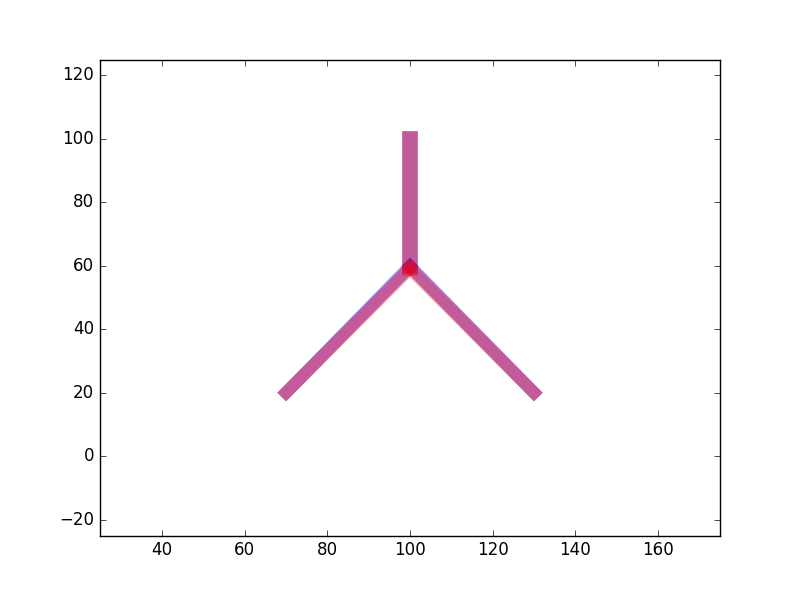
\includegraphics[width=0.45\textwidth]{./Images/Kamiya/Superposition_Firstandlast_t0.png}}
\subfigure[Random child locations and $Q_l = Q_r = \frac{1}{2} Q_p$]{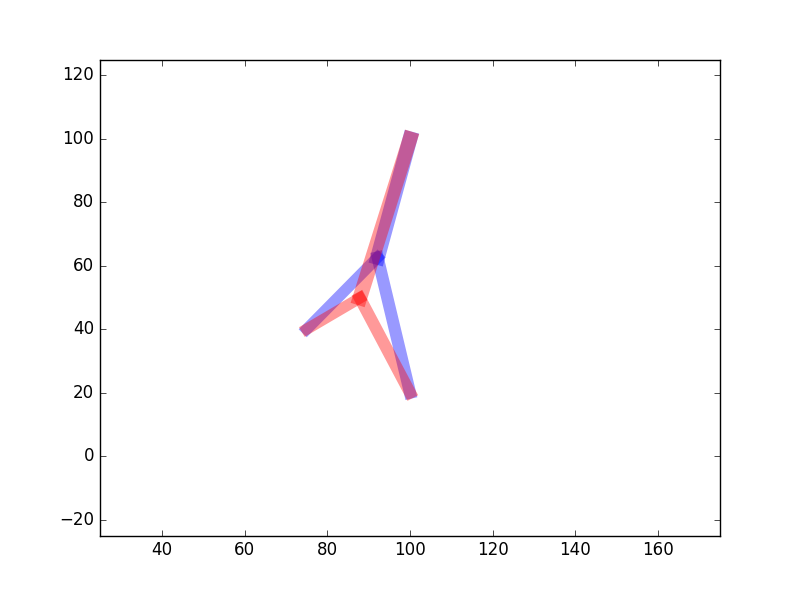
\includegraphics[width=0.45\textwidth]{./Images/Kamiya/Superposition_Firstandlast_t1.png} }\\
\subfigure[$Q_l = \frac{1}{4} Q_p$ and $Q_l = \frac{3}{4} Q_p$]{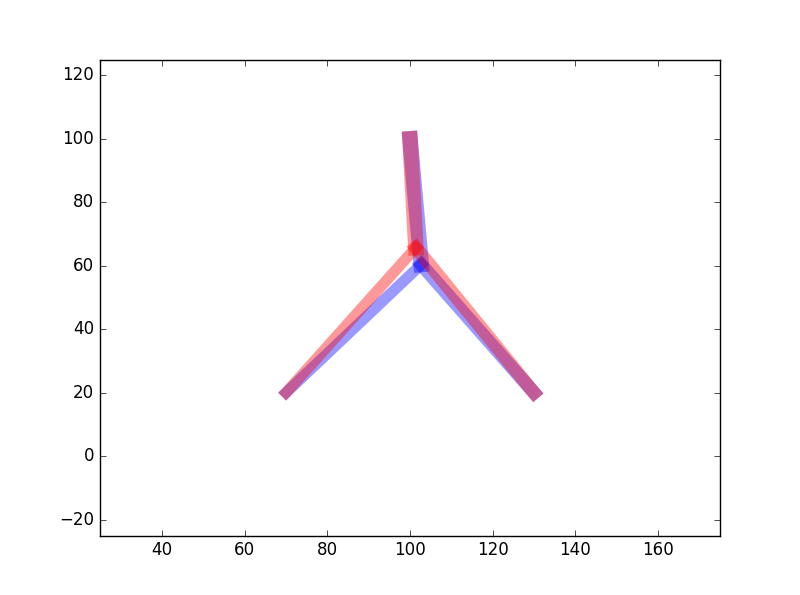
\includegraphics[width=0.45\textwidth]{./Images/Kamiya/Superposition_Firstandlast_t2.png} }
\subfigure[Random child locations and $Q_l = \frac{1}{4} Q_p$, $Q_l = \frac{3}{4} Q_p$]{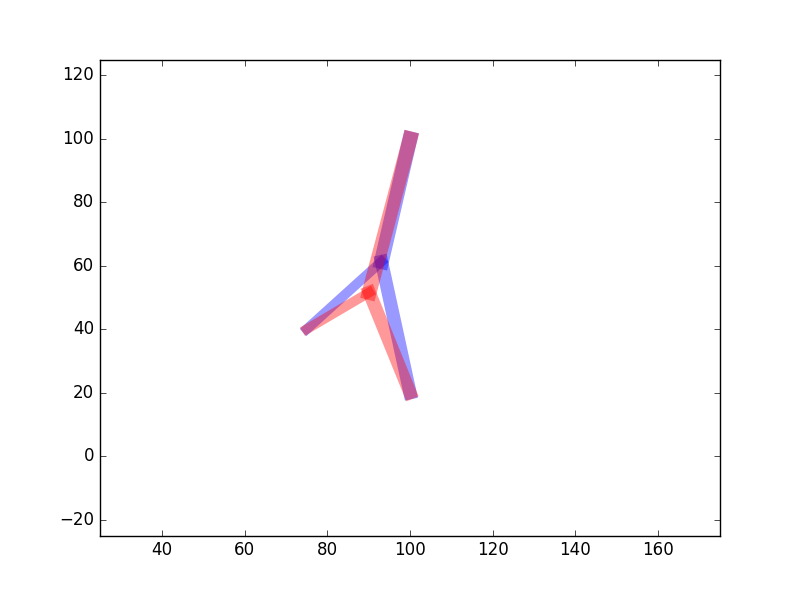
\includegraphics[width=0.45\textwidth]{./Images/Kamiya/Superposition_Firstandlast_t3.png} }

\caption{In blue the starting bifurcation (convex average position), in red the final bifurcation after Kamiya's algorithm convergence reached (tolerance = 0.01). Convergence was reached at 15th, 24th, 31st and 21st iteration respectively in (a),(b),(c),(d). $Q_p$ is the flow in parent branch, $Q_l$ and $Q_r$ are flows in left and right children.}
\label{fig:generation}
\end{figure}

\subsection*{Karch implementation}

Karch added lower and upper bounds to Kamiya's algorithm that ensures:
bifurcation position within the perfusion volume
the bifurcation not to degenerate to zero (by constraining segment length over segment diameter).


%------------------------------------------------

\section*{Conclusion}



\begin{appendices}
\section*{Equation \eqref{min volume}, from Kamiya \& Togawa 1972 equation  (6)}
Kamiya uses Murray definition at equation (7) from Physiological principle of minimum work\cite{murray1926physiological} that he calls the simplest requirement for efficiency in the circulation:
\begin{equation*}
f = k r^3
\end{equation*}
With k being a constant, so that the flow of blood past any section shall everywhere bear the same relation to the cube of the radius of the vessel at that point. Using it as:
\begin{equation*}
r_i^3 = \frac{r_i^6 k}{f_i}
\end{equation*}

and combining it this with the famous Murray's law,

\begin{equation*}
r_0^\gamma = r_1^\gamma + r_2^\gamma \text{ with } \gamma = 3
\end{equation*}

 where $r_0$ is the parent radius, $r_1$ and $r_2$ are the children radii, one obtains:
\begin{equation*}
\frac{k r_0^6}{f_0} = \frac{k r_1^6}{f_1} + \frac{k r_2^6}{f_2}
\end{equation*}
that can be simplified into equation \eqref{min volume}.


\section*{Equation \eqref{position}, from Kamiya \& Togawa 1972 equation  (7) }
We have
\begin{equation}
\label{eq:V}
V = \pi(r_0^2 l_0 + r_1^2 l_1 + r_2^2 l_2)
\end{equation}

and
\begin{align*}
l_0^2 &= \sqlen{0} \\
l_1^2 &= \sqlen{1} \\
l_2^2 &= \sqlen{2} 
\end{align*}

We rewrite \eqref{eq:V}

\begin{equation*}
V = \pi(r_0^2 \sqrt{\sqlen{0}} + r_1^2 \sqrt{\sqlen{1}} + r_2^2 \sqrt{\sqlen{2}})
\end{equation*}

We derive each term with respect to $x$.

\begin{equation*}
\frac{\partial}{\partial x} \sqrt{\sqlen{0}} = \frac{x-x_0}{\sqrt{\sqlen{0}}} = \frac{x-x_0}{l_0},
\end{equation*}
same for the $x_1$ and $x_2$ term, so we have

\begin{equation*}
\frac{\partial V}{\partial x} = \pi\left[ \frac{r_0^2(x-x_0)}{l_0} + \frac{r_1^2(x-x_1)}{l_1} + \frac{r_2^2(x-x_2)}{l_2}\right] = 0
\end{equation*}

Discarding the $\pi$ factor and separating the terms,

\begin{align*}
x\rili{0} + x\rili{1} + x\rili{2} &= x_0\rili{0} + x_1\rili{1} + x_2\rili{2} \\
x(\rili{0} + \rili{1} + \rili{2}) &= x_0\rili{0} + x_1\rili{1} + x_2\rili{2} 
\end{align*}

and so

\begin{equation*}
x = \frac{x_0\rili{0} + x_1\rili{1} + x_2\rili{2}}{\rili{0} + \rili{1} + \rili{2}}
\end{equation*}

This is one half of Eq.(7) in Kamiya \& Togawa. The other half is obtained by substituting $x$ with $y$ everywhere. This is
correct but not 100\% satisfying since the $l_i$ depend on $x$ and $y$.

\end{appendices}

%----------------------------------------------------------------------------------------
%	BIBLIOGRAPHY
%----------------------------------------------------------------------------------------

\bibliographystyle{unsrt}

\bibliography{sample}

%----------------------------------------------------------------------------------------

\end{document}